% Options for packages loaded elsewhere
\PassOptionsToPackage{unicode}{hyperref}
\PassOptionsToPackage{hyphens}{url}
\PassOptionsToPackage{dvipsnames,svgnames*,x11names*}{xcolor}
%
\documentclass[
]{book}
\usepackage{lmodern}
\usepackage{amssymb,amsmath}
\usepackage{ifxetex,ifluatex}
\ifnum 0\ifxetex 1\fi\ifluatex 1\fi=0 % if pdftex
  \usepackage[T1]{fontenc}
  \usepackage[utf8]{inputenc}
  \usepackage{textcomp} % provide euro and other symbols
\else % if luatex or xetex
  \usepackage{unicode-math}
  \defaultfontfeatures{Scale=MatchLowercase}
  \defaultfontfeatures[\rmfamily]{Ligatures=TeX,Scale=1}
\fi
% Use upquote if available, for straight quotes in verbatim environments
\IfFileExists{upquote.sty}{\usepackage{upquote}}{}
\IfFileExists{microtype.sty}{% use microtype if available
  \usepackage[]{microtype}
  \UseMicrotypeSet[protrusion]{basicmath} % disable protrusion for tt fonts
}{}
\makeatletter
\@ifundefined{KOMAClassName}{% if non-KOMA class
  \IfFileExists{parskip.sty}{%
    \usepackage{parskip}
  }{% else
    \setlength{\parindent}{0pt}
    \setlength{\parskip}{6pt plus 2pt minus 1pt}}
}{% if KOMA class
  \KOMAoptions{parskip=half}}
\makeatother
\usepackage{xcolor}
\IfFileExists{xurl.sty}{\usepackage{xurl}}{} % add URL line breaks if available
\IfFileExists{bookmark.sty}{\usepackage{bookmark}}{\usepackage{hyperref}}
\hypersetup{
  colorlinks=true,
  linkcolor=Maroon,
  filecolor=Maroon,
  citecolor=Blue,
  urlcolor=blue,
  pdfcreator={LaTeX via pandoc}}
\urlstyle{same} % disable monospaced font for URLs
\usepackage{color}
\usepackage{fancyvrb}
\newcommand{\VerbBar}{|}
\newcommand{\VERB}{\Verb[commandchars=\\\{\}]}
\DefineVerbatimEnvironment{Highlighting}{Verbatim}{commandchars=\\\{\}}
% Add ',fontsize=\small' for more characters per line
\usepackage{framed}
\definecolor{shadecolor}{RGB}{248,248,248}
\newenvironment{Shaded}{\begin{snugshade}}{\end{snugshade}}
\newcommand{\AlertTok}[1]{\textcolor[rgb]{0.94,0.16,0.16}{#1}}
\newcommand{\AnnotationTok}[1]{\textcolor[rgb]{0.56,0.35,0.01}{\textbf{\textit{#1}}}}
\newcommand{\AttributeTok}[1]{\textcolor[rgb]{0.77,0.63,0.00}{#1}}
\newcommand{\BaseNTok}[1]{\textcolor[rgb]{0.00,0.00,0.81}{#1}}
\newcommand{\BuiltInTok}[1]{#1}
\newcommand{\CharTok}[1]{\textcolor[rgb]{0.31,0.60,0.02}{#1}}
\newcommand{\CommentTok}[1]{\textcolor[rgb]{0.56,0.35,0.01}{\textit{#1}}}
\newcommand{\CommentVarTok}[1]{\textcolor[rgb]{0.56,0.35,0.01}{\textbf{\textit{#1}}}}
\newcommand{\ConstantTok}[1]{\textcolor[rgb]{0.00,0.00,0.00}{#1}}
\newcommand{\ControlFlowTok}[1]{\textcolor[rgb]{0.13,0.29,0.53}{\textbf{#1}}}
\newcommand{\DataTypeTok}[1]{\textcolor[rgb]{0.13,0.29,0.53}{#1}}
\newcommand{\DecValTok}[1]{\textcolor[rgb]{0.00,0.00,0.81}{#1}}
\newcommand{\DocumentationTok}[1]{\textcolor[rgb]{0.56,0.35,0.01}{\textbf{\textit{#1}}}}
\newcommand{\ErrorTok}[1]{\textcolor[rgb]{0.64,0.00,0.00}{\textbf{#1}}}
\newcommand{\ExtensionTok}[1]{#1}
\newcommand{\FloatTok}[1]{\textcolor[rgb]{0.00,0.00,0.81}{#1}}
\newcommand{\FunctionTok}[1]{\textcolor[rgb]{0.00,0.00,0.00}{#1}}
\newcommand{\ImportTok}[1]{#1}
\newcommand{\InformationTok}[1]{\textcolor[rgb]{0.56,0.35,0.01}{\textbf{\textit{#1}}}}
\newcommand{\KeywordTok}[1]{\textcolor[rgb]{0.13,0.29,0.53}{\textbf{#1}}}
\newcommand{\NormalTok}[1]{#1}
\newcommand{\OperatorTok}[1]{\textcolor[rgb]{0.81,0.36,0.00}{\textbf{#1}}}
\newcommand{\OtherTok}[1]{\textcolor[rgb]{0.56,0.35,0.01}{#1}}
\newcommand{\PreprocessorTok}[1]{\textcolor[rgb]{0.56,0.35,0.01}{\textit{#1}}}
\newcommand{\RegionMarkerTok}[1]{#1}
\newcommand{\SpecialCharTok}[1]{\textcolor[rgb]{0.00,0.00,0.00}{#1}}
\newcommand{\SpecialStringTok}[1]{\textcolor[rgb]{0.31,0.60,0.02}{#1}}
\newcommand{\StringTok}[1]{\textcolor[rgb]{0.31,0.60,0.02}{#1}}
\newcommand{\VariableTok}[1]{\textcolor[rgb]{0.00,0.00,0.00}{#1}}
\newcommand{\VerbatimStringTok}[1]{\textcolor[rgb]{0.31,0.60,0.02}{#1}}
\newcommand{\WarningTok}[1]{\textcolor[rgb]{0.56,0.35,0.01}{\textbf{\textit{#1}}}}
\usepackage{longtable,booktabs}
% Correct order of tables after \paragraph or \subparagraph
\usepackage{etoolbox}
\makeatletter
\patchcmd\longtable{\par}{\if@noskipsec\mbox{}\fi\par}{}{}
\makeatother
% Allow footnotes in longtable head/foot
\IfFileExists{footnotehyper.sty}{\usepackage{footnotehyper}}{\usepackage{footnote}}
\makesavenoteenv{longtable}
\usepackage{graphicx}
\makeatletter
\def\maxwidth{\ifdim\Gin@nat@width>\linewidth\linewidth\else\Gin@nat@width\fi}
\def\maxheight{\ifdim\Gin@nat@height>\textheight\textheight\else\Gin@nat@height\fi}
\makeatother
% Scale images if necessary, so that they will not overflow the page
% margins by default, and it is still possible to overwrite the defaults
% using explicit options in \includegraphics[width, height, ...]{}
\setkeys{Gin}{width=\maxwidth,height=\maxheight,keepaspectratio}
% Set default figure placement to htbp
\makeatletter
\def\fps@figure{htbp}
\makeatother
\setlength{\emergencystretch}{3em} % prevent overfull lines
\providecommand{\tightlist}{%
  \setlength{\itemsep}{0pt}\setlength{\parskip}{0pt}}
\setcounter{secnumdepth}{5}
\usepackage{booktabs}

\newenvironment{rmdblock}[1]
  {\begin{shaded*}
  \begin{itemize}
  \renewcommand{\labelitemi}{
    \raisebox{-.7\height}[0pt][0pt]{
      {\setkeys{Gin}{width=2em,keepaspectratio}\includegraphics{image/#1}}
    }
  }
  \item
  }
  {
  \end{itemize}
  \end{shaded*}
  }
\newenvironment{rmdas}
  {\begin{rmdblock}{as}}
  {\end{rmdblock}}
\newenvironment{rmdvd}
  {\begin{rmdblock}{vd}}
  {\end{rmdblock}}
\newenvironment{rmdrd}
  {\begin{rmdblock}{rd}}
  {\end{rmdblock}}

%\usepackage{color}
\usepackage{pdfpages}

% \usepackage{xeCJK}
\AtBeginDocument{\renewcommand{\chaptername}{Week}}
\usepackage[]{natbib}
\bibliographystyle{apalike}

\author{}
\date{\vspace{-2.5em}}

\begin{document}


\includepdf[pages=-]{image/cover.pdf}

\thispagestyle{empty}

\setlength{\abovedisplayskip}{-5pt}
\setlength{\abovedisplayshortskip}{-5pt}

{
\hypersetup{linkcolor=}
\setcounter{tocdepth}{1}
\tableofcontents
}
\frontmatter

\hypertarget{preface}{%
\chapter{Preface}\label{preface}}

This is a short guide for new staff at Xi'an Jiaotong-Livepool University. All these contents are extracted from XJTLU's regulations or the author's experience.

I try to update this book frequently, while I take no responsibility and assumes no liability for any content in this book.

\begin{rmdrd}
A block like this is reading materials.
\end{rmdrd}

\begin{rmdas}
A block like this is a form.
\end{rmdas}

\begin{rmdvd}
A block like this is a video.
\end{rmdvd}

This book is created with the R package bookdown. The session information is as follows:

\begin{Shaded}
\begin{Highlighting}[]
\KeywordTok{sessionInfo}\NormalTok{()}
\end{Highlighting}
\end{Shaded}

\begin{verbatim}
## R version 4.0.1 (2020-06-06)
## Platform: x86_64-w64-mingw32/x64 (64-bit)
## Running under: Windows 10 x64 (build 19041)
## 
## Matrix products: default
## 
## locale:
## [1] LC_COLLATE=Chinese (Simplified)_China.936 
## [2] LC_CTYPE=Chinese (Simplified)_China.936   
## [3] LC_MONETARY=Chinese (Simplified)_China.936
## [4] LC_NUMERIC=C                              
## [5] LC_TIME=Chinese (Simplified)_China.936    
## 
## attached base packages:
## [1] stats     graphics  grDevices utils     datasets 
## [6] methods   base     
## 
## loaded via a namespace (and not attached):
##  [1] compiler_4.0.1  magrittr_1.5    bookdown_0.20  
##  [4] tools_4.0.1     htmltools_0.5.0 rstudioapi_0.11
##  [7] yaml_2.2.1      stringi_1.4.6   rmarkdown_2.3  
## [10] knitr_1.29      stringr_1.4.0   xfun_0.16      
## [13] digest_0.6.25   rlang_0.4.7     evaluate_0.14
\end{verbatim}

The R packages used in this book are:

\begin{verbatim}
## [1] "RefManageR"
\end{verbatim}

\mainmatter

\hypertarget{general-introduction}{%
\chapter{General introduction}\label{general-introduction}}

\hypertarget{reading-materials}{%
\section{Reading materials}\label{reading-materials}}

\begin{itemize}
\tightlist
\item
  \href{https://box.xjtlu.edu.cn/\#common/lib/633bf817-899c-4be7-ab42-1d4986349f4c/New\%20Staff\%20Induction}{New Staff Induction: General}
\item
  \href{https://box.xjtlu.edu.cn/\#common/lib/76a264ad-c956-4ed2-abd7-7088081fe1fd/}{New Staff Induction: Academic}
\item
  \href{https://box.xjtlu.edu.cn/smart-link/1d9f1e2d-39e6-46de-b46f-e459502ed6df/}{Staff Handbook}
\item
  \href{https://box.xjtlu.edu.cn/smart-link/88e4699f-4ee6-43aa-a83d-0c86c1589818/}{Legal Stay in China} (Tips for Foreign Staff)
\item
  \href{https://box.xjtlu.edu.cn/smart-link/f7764aa3-7a36-40a7-bf2d-47f8bc57b1e7/}{Staff Directory} (Updated on a regular basis)
\item
  \href{https://box.xjtlu.edu.cn/smart-link/1999109a-e714-4ada-ade1-4785e256b15d/}{Tax Rate} (Individual Income Tax)
\item
  \href{https://box.xjtlu.edu.cn/smart-link/27acb50a-1e80-46df-843a-a944d36764d5/}{Payroll Processing Schedule}
\item
  \href{https://www.expat.com/en/destination/asia/china/}{Living in China}
\item
  \href{https://connect.xjtlu.edu.cn/user/td-hr/hr-monthly-newsletter-december-2019}{HR Monthly Newsletter}
\item
  XJTLU Brochure for Working on Campus (\href{https://box.xjtlu.edu.cn/smart-link/50c776fc-eec7-4219-a03b-eca4ad1d577f/}{English}, \href{https://box.xjtlu.edu.cn/smart-link/e678f16a-a01e-44ba-87f2-4cddf3bc2c23/}{Chinese})
\end{itemize}

\hypertarget{covid-19}{%
\section{COVID-19}\label{covid-19}}

\begin{itemize}
\tightlist
\item
  24-hour Hotlines for Expats in SIP

  \begin{itemize}
  \tightlist
  \item
    English: 0512-66681812/13771835783
  \item
    Japanese: 0512-66681529/13914086240\\
  \item
    Korean: 0512-66681802/18626205975
  \end{itemize}
\item
  \href{https://www.xjtlu.edu.cn/en/novel-coronavirus-pneumonia/useful-tips-and-reminding/}{University useful Tips and Reminding}
\item
  \href{http://weekly.chinacdc.cn/index.htm}{China CDC (Chinese Center for Disease Control and Prevention}\href{http://weekly.chinacdc.cn/index.htm}{) Weekly}
\end{itemize}

\hypertarget{work}{%
\chapter{Work}\label{work}}

\hypertarget{faculty-report}{%
\section{Faculty report}\label{faculty-report}}

A faculty report was suggested by Prof.~Johannes Knops as an annual summary, which serves as a guideline for the work. The structure of the report is illustrated in Fig. \ref{fig:report}.

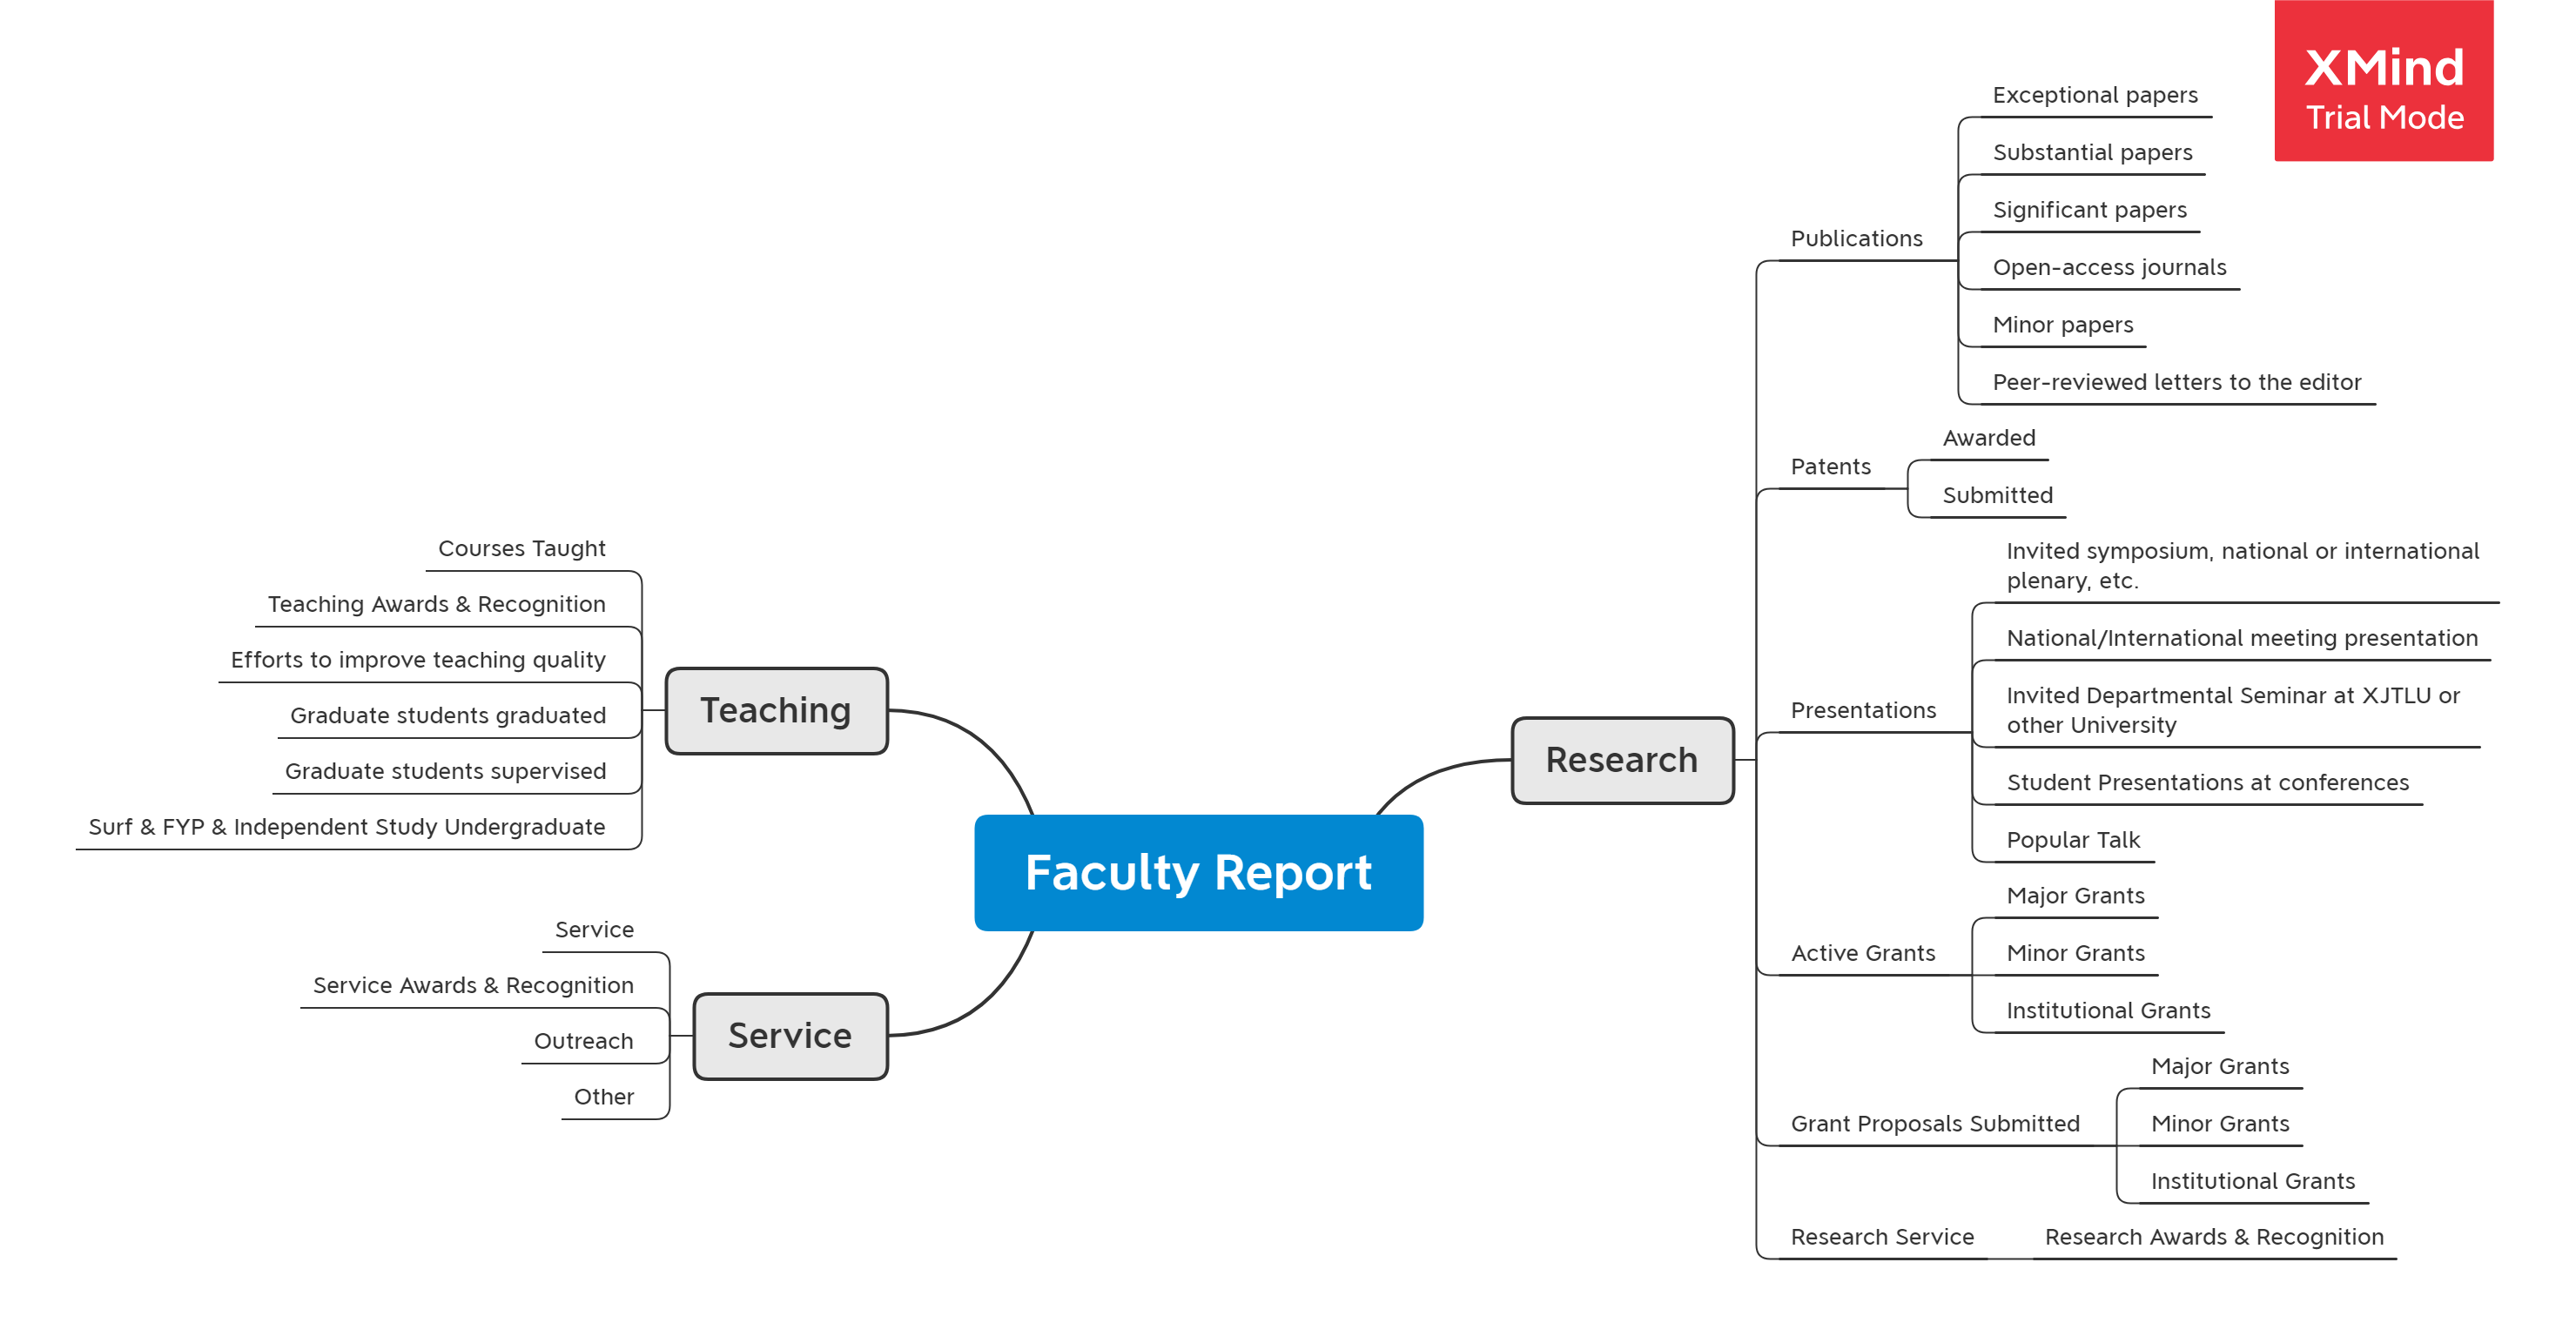
\includegraphics{image/faculty_report.png}

Figure \label{fig:report}. Recommended structure of a faculty report.

A template of this report is available in the R package ``xjtlu''.

\hypertarget{teaching}{%
\section{Teaching}\label{teaching}}

\begin{itemize}
\tightlist
\item
  \href{https://ice.xjtlu.edu.cn/course/view.php?id=1605\&section=1}{Marking and Moderation}
\end{itemize}

\hypertarget{collaboration}{%
\section{Collaboration}\label{collaboration}}

Research Office produced a video about how to draft appropriate technology agreement when starting cooperation with external enterprise or other organizations in XJTLU. The video can be found \href{https://box.xjtlu.edu.cn/smart-link/d0dc536d-1b5f-4a75-bcce-087a14a929ad/}{here}.

\hypertarget{library}{%
\chapter{Library}\label{library}}

\hypertarget{location-and-opening-hours}{%
\section{Location and opening hours}\label{location-and-opening-hours}}

Location: Central Building, Level 1, 3 -- 10, 22,000 m\textsuperscript{2}, 2,800 seats and 300 computer terminals.

Opening hours:

\begin{itemize}
\item
  Monday- Friday: 8:00 -- 22:00
\item
  Saturday and Sunday: 9:00 -- 22:00
\end{itemize}

For summer and winter holidays, the opening hours will be pre-announced via e-mail and posted at the entrance of the library.

\hypertarget{borrow-books}{%
\section{Borrow books}\label{borrow-books}}

Search books on \url{http://opac.lib.xjtlu.edu.cn}。

With your university ID card, books can be checked out or returned either at self-service machines on the 1st, 4th and 8th floors, or at the Library Circulation Desk on the 3rd floor.

For CDs, DVDs, course reserves and reserved books, please return them to the Library Circulation Desk on the 3rd floor.

Academic staff can keep unlimited books for 180 days, DVDs and short loan for 3 days, and graded readers for 7 days. Academic staff have unlimited renewals on borrowed books. T

\hypertarget{remote-access}{%
\section{Remote access}\label{remote-access}}

\begin{rmdvd}
\begin{itemize}
\tightlist
\item
  \href{https://box.xjtlu.edu.cn/smart-link/9d8e7934-d6eb-4400-9285-8f6c14933ed9/}{Tutorial:videos on how to access library services and resources remotely}
\end{itemize}
\end{rmdvd}

\hypertarget{book-purchase}{%
\section{Book purchase}\label{book-purchase}}

If you would like our library to buy some books for your teaching or research, there are three ways you could choose:

\begin{enumerate}
\def\labelenumi{\arabic{enumi}.}
\item
  \textbf{The library buys books for you}. Fill in the \href{http://libguides.lib.xjtlu.edu.cn/ld.php?content_id=15552390}{Purchase\_Request\_Form.xls} with your book info, and send the form to the library officer. No need to print it out or scan it. The Excel form is fine. The library officer will forward it to our library. The purchase takes one or two months. More details can be found in the \href{http://libguides.lib.xjtlu.edu.cn/ld.php?content_id=15552051}{Policy on Print Book Collection Development}.
\item
  \textbf{You buy books by yourself and get reimbursement from the library.} \textbf{Before you buy books}, you have to fill the \href{https://libguides.lib.xjtlu.edu.cn/ld.php?content_id=47964273}{Staff\_Reimbursement\_Request\_Form.xls}, and send it to the library officer. You will get the reimbursement, and you have to bring the books to the library for the library stamps. More details can be found in the\href{http://libguides.lib.xjtlu.edu.cn/ld.php?content_id=15552277}{Library Policy on Staff Self-Purchase Reimbursement}.
\item
  You could also buy books at the Eslite (Chengpin) Bookstore, Phoenix (Fenghuang) Bookstore, Xinhua

  Bookstore in Guanqian Street, which have some agreements with our library. The payment will go to our library directly.
\end{enumerate}

The books bought in these three ways will be stored in our library.

\begin{rmdrd}
\begin{itemize}
\tightlist
\item
  \href{https://libguides.lib.xjtlu.edu.cn/c.php?g=376964\&p=6685926}{How to Suggest a Purchase}
\item
  \href{http://libguides.lib.xjtlu.edu.cn/ld.php?content_id=15552051}{Policy on Print Book Collection Development}
\item
  \href{http://libguides.lib.xjtlu.edu.cn/ld.php?content_id=15552277}{Library Policy on Staff Self-Purchase Reimbursement}
\end{itemize}
\end{rmdrd}

\hypertarget{textbooks}{%
\section{Textbooks}\label{textbooks}}

Module leaders should provide accurate and complete information (including ISBN, title, author, publisher) for the textbook via e-Bridge within the specified deadline.

Module leaders/conveners are entitled to free textbook desk copies from Textbook and Publication Division by the following two ways:

\begin{itemize}
\tightlist
\item
  Collecting it from Library in person one week before new semester begins;
\item
  Contacting publishers directly if the Desk Copy is needed before the time stated above.
\end{itemize}

There are three categories of textbook: Mandatory Textbook, Optional Textbook and Reference Textbook.

\begin{enumerate}
\def\labelenumi{\arabic{enumi}.}
\tightlist
\item
  MANDATORY: A required book in either print or electronic format for a module that students are obligated to purchase.
\item
  OPTIONAL: A book in print that students can choose to purchase or not.
\item
  REFERENCE: A book in print that is considered additional or recommended reading by academic staff and is only purchased for Library's collection where it can be offered for loan.
\end{enumerate}

\hypertarget{group-study-room-and-training-room}{%
\section{Group Study Room and Training Room}\label{group-study-room-and-training-room}}

Group Study Rooms (Room 314, 316, 318, 429, 445, 545, 547, 714 and 814) aim to provide students and staff space for group discussion within the library upon booking. Each person can only book a room once a day. Booking is limited to a maximum of 3 hours for students and 6 hours for staff. Room booking can be done via \href{http://bookings.lib.xjtlu.edu.cn}{Library Room Booking System} and can be booked up to 7 days in advance.

Library Training Room 303 has 1 computer, 1 projector and 1 moveable whiteboard, with a capacity of 48 people. Reservation can be made via \href{http://mrbs.xjtlu.edu.cn/day.php}{XJTLU Room Booking system} by staff for teaching activities.

\hypertarget{training}{%
\section{Training}\label{training}}

Library information literacy education schedule can be found in LibCal (library calendar for training and student activities) at \url{http://libcal.lib.xjtlu.edu.cn}. For further queries and suggestions, please email \href{mailto:libtraining@xjtlu.edu.cn}{\nolinkurl{libtraining@xjtlu.edu.cn}}.

Learning in Virtual Environment (\href{http://vle.lib.xjtlu.edu.cn}{LiVE}) is the Library's e-learning platform which provides information and research skills online trainings. You can login with your university account and take different modules in LiVE to learn about information searching, referencing, digital library usage, etc.

\hypertarget{publishing-books}{%
\section{Publishing books}\label{publishing-books}}

XJTLU has established XJTLU IMPRINT, an academic publisher that is a sub-division of Liverpool University Press.

As a leading joint-venture university in China, XJTLU is ideally placed to become world-leading in intellectual exchange between China and the rest of the world. A central aim of the XJTLU IMPRINT is to support this mission and facilitate academic dialogue between China and the Anglophone world.

XJTLU IMPRINT launches a Call for proposal for publications. The proposals of publications may include (but are not limited to):

\begin{itemize}
\tightlist
\item
  Original research monographs
\item
  Edited volumes
\item
  Journals
\item
  Conference Proceedings\\
\item
  Textbooks
\item
  Translations of impactful Chinese academic works into English
\item
  Translations of impactful English academic works into Chinese
\item
  Bilingual articles\\
\item
  Creative works, e.g.~screenplays
\end{itemize}

All submissions will be subject to internal and external review.

XJTLU IMPRINT will seek to prioritise work that either speaks to the theme of intercultural exchange, that widens the reach of research in the areas of Humanities, Sciences, Technologies, and Social Sciences by being presented in a bilingual format, or that takes an innovative pedagogical perspective appropriate to a global context.

Contact: \href{mailto:editorial@xjtlu.edu.cn}{\nolinkurl{editorial@xjtlu.edu.cn}}, \href{mailto:publishingcommittee@xjtlu.edu.cn}{\nolinkurl{publishingcommittee@xjtlu.edu.cn}}

\hypertarget{cmo-campus-management-office}{%
\chapter{CMO (Campus Management Office)}\label{cmo-campus-management-office}}

\hypertarget{how-to-make-phone-calls}{%
\section{How to make phone calls}\label{how-to-make-phone-calls}}

\begin{itemize}
\tightlist
\item
  Dial the four digital number for internal calls.
\item
  Dial ``9'' before the phone number for Suzhou calls.
\item
  Dial ``90'' before the phone number for those outside of Suzhou.
\end{itemize}

\hypertarget{household-waste-classification-and-disposal}{%
\section{Household Waste Classification and Disposal}\label{household-waste-classification-and-disposal}}

The Recyclable, Residual, and Food waste containers are in staff common rooms, student common rooms, tea rooms and corridors in each building on campus, except that the hazardous waste containers are near the Property Management Office or near the entrances \& exits in each building.

\begin{itemize}
\tightlist
\item
  Recyclable: mainly include mental, glass products, radios, cell phones, newspaper cardboards cases, clothing bedding, plastic, etc.
\item
  Residual Waste: mainly include disposable dry cells labeled with `no mercury', used toilet paper, cigarette butts, instant-noodle boxes, disposable cups, etc.
\item
  Food Waste: mainly include expired cooking oil, fruits peels, fallen leaves, leftovers scraps, etc.
\item
  Hazardous Waste: mainly include fluorescent bulbs exergy-saving bulbs, paint cans, phone batteries button cells, mercury thermometer, pesticide, expired medicine, etc.
\end{itemize}

\hypertarget{it}{%
\chapter{IT}\label{it}}

\hypertarget{request-hardware-and-software}{%
\section{Request hardware and software}\label{request-hardware-and-software}}

\begin{enumerate}
\def\labelenumi{\arabic{enumi}.}
\tightlist
\item
  Requestor submits a completed IT Request Form to MITS to assess and confirm solution.
\end{enumerate}

\begin{itemize}
\tightlist
\item
  \href{https://box.xjtlu.edu.cn/lib/b1e91eec-7498-438e-823c-a6d3ba1727f6/file/Forms/Form-IT\%20Assets\%20Request-Hardware\%20and\%20Rebuilding.doc}{IT Hardware/Rebuilding Request Form}
\item
  \href{https://box.xjtlu.edu.cn/lib/b1e91eec-7498-438e-823c-a6d3ba1727f6/file/Forms/Form-IT\%20Assets\%20Request-Software.doc}{IT Software Request Form}
  Note: the general IT Consumable/Digital Product is centralized by MITS budget such as keyboard, Mouse, Computer Camera, portable hard disk, laser pen\ldots\ldots{}
\end{itemize}

\begin{enumerate}
\def\labelenumi{\arabic{enumi}.}
\setcounter{enumi}{1}
\tightlist
\item
  MITS submits an approved CMO01 form to the Sourcing and Purchasing Office.
\item
  Sourcing and Purchasing Office complete their internal Purchasing Process.
\item
  MITS assists by installing, supporting, or providing maintenance as needed.
\end{enumerate}

\begin{rmdrd}
\begin{itemize}
\tightlist
\item
  \href{https://box.xjtlu.edu.cn/lib/883faf64-eff0-432e-8426-462815438e4c/file/UC/UC\%20for\%20Staff/201910/Notice/Procurement\%20Management\%20Policy.pdf}{XJTLU Procurement Management Policy}
\item
  \href{https://box.xjtlu.edu.cn/smart-link/985f3f45-5d2c-4aff-8b83-0f117692e508/}{MITS Reminder Purchase Procedure for IT Hardware and Software}
\end{itemize}
\end{rmdrd}

\hypertarget{vpn}{%
\section{VPN}\label{vpn}}

XJTLU staff and students are able to access intranet resources off-campus by using a VPN (Virtual Private

Network).

\textbf{Instructions for Windows 7/10:}

\begin{enumerate}
\def\labelenumi{\arabic{enumi}.}
\tightlist
\item
  Double click the installation file ``vpnclient-***.exe'' file and run it for installation. During the installation, Select ``PacketiX VPN Client''.
\item
  After the installation, start the PacketiX VPN Client Manager.
\item
  Double click ``Add VPN Connection''. Click ``Yes''. Click ``OK''.
\item
  The Virtual Network Adapter you created will then shown in the lower window, for example as shown below ``VPN Client Adapter - VPN'', double click ``Add VPN Connection'' in the upper window again.
\item
  Fill the details as shown below in the ``New VPN Connection Setting Properties'' and click ``OK''.

  \begin{itemize}
  \tightlist
  \item
    Setting Name: New VPN Connection (default name generated automatically)
  \item
    Host Name: vpn.xjtlu.edu.cn
  \item
    Port Number: 5555
  \item
    Virtual Hub Name: aaa (You must set `Host Name' and `Port Number' first)
  \item
    Auth Type: RADIUS or NT Domain Authentication
  \item
    User Name: \emph{Your username}
  \item
    Password: \emph{Your password}
  \end{itemize}
\item
  The ``New VPN Connection'' is shown in the upper window. Double click on ``New VPN Connection'', the status will show as ``Connected''.
\item
  Right-click on ``New VPN Connection'' and click ``Disconnect'' when you want to leave the intranet. Click ``Remove Startup Connection'' to prevent automatic connection when you power on your computer.
\end{enumerate}

\textbf{Instructions for Mac OS:}

\begin{enumerate}
\def\labelenumi{\arabic{enumi}.}
\item
  Click ``Network'' in System Preferences.
\item
  Add an interface ``VPN''.
\item
  Select VPN Type ``L2TP over IPSec'', set up a Service Name ``VPN (L2TP)'', then click ``Create''.
\item
  Add Configuration Name ``vpn-test'', then click ``Create''.
\item
  Add the Server Address: ``vpn.xjtlu.edu.cn'' and ``\emph{Your Account Name}'', then click ``Authentication
\end{enumerate}

Settings\ldots''

\begin{enumerate}
\def\labelenumi{\arabic{enumi}.}
\setcounter{enumi}{5}
\tightlist
\item
  Fill in your Password (optional) and Shared Secret ``vpn'', then click ``OK''.
\item
  Click ``Advanced\ldots{}''.
\item
  Make sure all the first 3 boxes in the ``Options'' tab are all ticked and click ``OK''.
\item
  Click ``Apply'', then ``Connect''. The connection will be established if you input your correct password in step 6, otherwise, a credential authentication window will pop up to ask for your password, fill with your password and then click ``OK''.
\item
  The Status will show as ``Connected'' if it authenticates successfully. Tick the box ``Show VPN status
\end{enumerate}

in menu bar''.

\textbf{Instruction for IOS:}

\begin{enumerate}
\def\labelenumi{\arabic{enumi}.}
\tightlist
\item
  Tap ``Settings''.
\item
  Tap ``General''.
\item
  Tap ``VPN''.
\item
  Tap ``Add VPN Configuration''.
\item
  Fill the details.
\item
  Slide the button to the right for connecting.
\item
  It will ask for password if you didn't provide in step 5.
\item
  The status will change as ``Connected''
\end{enumerate}

\textbf{Instruction for Andriod:}

The menu of android devices could be different according to different brands, here is an example for

HUAWEI phone.

\begin{enumerate}
\def\labelenumi{\arabic{enumi}.}
\tightlist
\item
  Find ``VPN'' in Wireless \& networks.
\item
  Tap ``Add VPN network''.
\item
  Fill the details and ``SAVE''.
\item
  Enter your credential and click ``CONNECT''. The status will change to ``Connected''.
\end{enumerate}

\hypertarget{how-to-make-videos}{%
\section{How to make videos}\label{how-to-make-videos}}

\begin{rmdvd}
\url{https://video.xjtlu.edu.cn/Mediasite/Play/d8e1d78569ff48778dfe198a669906261d}
\end{rmdvd}

\hypertarget{ice}{%
\section{ICE}\label{ice}}

The ICE Support Clinic provides one-to-one guidance and assistance daily from 15:00-16:00. Click \href{https://ice.xjtlu.edu.cn/mod/page/view.php?id=142089}{here}.

Recordings of online training sessions are available \href{https://ice.xjtlu.edu.cn/mod/glossary/view.php?id=128625}{here}.

\href{https://ice.xjtlu.edu.cn/course/view.php?id=1631}{Online Quiz Standardisation Module} teaches staff about the ICE's Quiz activity.

Podcasts about the XJTLU Experience during COVID-19 for UoL Staff are available \href{https://connect.xjtlu.edu.cn/view/view.php?t=kD90XzHKFxeqnty1Ppvc}{here}.

As a reminder, several ICE and BigBlueButton user guides related to a variety of features are available via the \href{https://ice.xjtlu.edu.cn/course/view.php?id=1605}{Online Learning and Teaching Technology Support} page. There is also an \href{https://ice.xjtlu.edu.cn/course/view.php?id=1605\&section=17}{FAQ/Support forum}.

\hypertarget{uol}{%
\section{UoL}\label{uol}}

\href{https://www.liverpool.ac.uk/csd/fundamentals/}{IT Fundamentals for staff}

\hypertarget{matlab}{%
\section{MatLab}\label{matlab}}

\begin{itemize}
\tightlist
\item
  \href{https://guide.xjtlu.edu.cn/how-to-register-and-install-matlab-license-for-student.html}{MATLAB License Registration and Installation Guide (For student)}
\item
  \href{https://guide.xjtlu.edu.cn/how-to-register-and-install-matlab-license-for-staff.html}{MATLAB License Registration and Installation Guide (For staff)}
\item
  \href{https://matlabacademy.mathworks.co}{MATLAB and Simulink online coursesportal}
\end{itemize}

\hypertarget{financial}{%
\chapter{Financial}\label{financial}}

\hypertarget{fapiao}{%
\section{Fapiao}\label{fapiao}}

\begin{center}
\includegraphics[width=0.8\linewidth]{image/fapiao} \end{center}

\end{document}
